\documentclass[norsk]{article}
\usepackage{babel}[norsk]
\usepackage[utf8]{inputenc}


\usepackage{amsthm}
\usepackage{amsmath}
\usepackage{amssymb}
\usepackage{enumitem}
\usepackage{tikz,pgflibraryarrows,pgflibraryplotmarks,pgflibrarysnakes,pgflibraryshapes}
\usepackage{tikzsymbols}
\usepackage{tikz-cd}
\usepackage{biblatex}[backend=biber]
\usepackage{graphicx}
\usepackage[keys, sets, operators, primitives]{cryptocode}


\usepackage{pgfplots}

\newtheorem{teorem}{Teorem}[section]
\newtheorem{proposisjon}[teorem]{Proposisjon}
\newtheorem{lemma}[teorem]{Lemma}
\newtheorem{korollar}[teorem]{Korollar}

\theoremstyle{definition}
\newtheorem{eksempel}[teorem]{Eksempel}
\newtheorem{definisjon}[teorem]{Definisjon}

\title{Bacheloroppgave}
\author{Jørgen}
\date{\today}


\newcommand{\R}{\mathbb{R}}
\newcommand{\Affine}{\mathbb{A}}
\newcommand{\Projective}{\mathbb{P}}
\newcommand{\OO}{\mathcal{O}}


\bibliography{references}

\begin{document}

\maketitle

\tableofcontents

\newpage


\section{Algebra}
%\begin{definisjon}
%Vi sier at et polynom $f(x) \in R[X]$ er primitivt, dersom største felles divisor til koefissientene er en enhet i $R$.
%\end{definisjon}

\begin{teorem}
Sylow:
La $G$ være en endelig gruppe og $p$ være et primtall. Dersom $p^m$ deler $|G|$ har $G$ en undergruppe av orden $p^m$. \cite{algebra}
\end{teorem}

\begin{teorem}
\label{fundamentalteoremet}
Fundamentalteoremet av endeliggenererte abelske grupper:
La $A$ være en endelig-generert abelsk gruppe. Da kan $A$ dekomponeres som en direktesum av et endelig anatall sykliske grupper $C_i$. 
$$A = C_1 \oplus \ldots C_k $$ 
For bevis, se \cite{algebra}
\end{teorem}

\begin{teorem}
\label{finite abelian group}
La $A$ være en endelig abelsk gruppe. Da finnes det en unik liste heltall $m_1, \ldots m_k$ (alle større enn 1), slik at $|A| = m_1 \ldots m_2$, og $A \cong \ZZ_{m_1} \oplus \ldots \oplus \ZZ_{m_k}$

For bevis, se  \cite{algebra}(3.1)
\end{teorem}


\begin{definisjon}
La $K[X]$ være et integritetsområde over potensielt flere variable. Da er kvotientkroppen en utvidelse av $K[X]$ som danner en kropp med elementene $$ \{(f,g) \mid f,g \in K[X], g \neq 0 \}$$
Med følgende ekvivalensrelasjon
$(f,g) \sim (f',g') \Leftrightarrow fg' = sf'g $ for en $s \in K[X]$

Vi skriver ofte elementene $(f,g)$ som $\frac{f}{g}$
\end{definisjon}

\begin{definisjon}
La $G$ være en gruppe, og $a,b \in G$ være to elementer i gruppa. Vi sier at $a$ og $b$ er lineart uavhengige dersom $[n]a + [m]b = e \Rightarrow n = m = 0$ for $n, m \in \ZZ$. 

Der $[n]a$ = $\underbrace{a * \ldots * a}_\text{ $n$ ganger}$, og $[0]a = e$
\end{definisjon}

\begin{definisjon}
La $E$ være en kroppsutvidelse av $F$. Et element $\alpha \in E$ er \textbf{algebraisk} over $F$ dersom det finnes elementer $a_0, \ldots a_n$ i $F$ (ikke alle lik 0), slik at $$a_0 + a_1\alpha + \ldots a_n \alpha^n = 0$$
\end{definisjon}

\begin{definisjon}
La $E$ være en kroppsutvidelse av $F$. Vi sier at $E$ er en \textbf{transcendental utvidelse} dersom det finnes et element $x \in E$ som ikke er algebraisk i $F$.
\end{definisjon}

\begin{definisjon}
La $E$ være en kroppsutvidelse av $F$ som konstrueres av elementene $x_1, \ldots, x_n$. Altså er $E = F(x_1, \ldots, x_n)$. Da er \textbf{graden} til $E$ lik antall elementer, $grad(E) = n$.
\end{definisjon}

Litt mer galoaisteori, så kan grafen under forklares 

\begin{tikzcd}
K(V) &  \\
 & {K(\lambda_1, \ldots \lambda_n)} \arrow[lu, no head] \\
K \arrow[ru, no head] \arrow[uu, no head] & 
\end{tikzcd}



\begin{eksempel}
Polynomet $f(x,y) = y^2 - x^3 - Ax - B$ er irredusibelt over $\overline{\FF}_p$. 
\label{Elliptisk Kurve polynom}
\begin{proof}
Annta ad absurdum at $f(x,y)$ kan faktoriseres. Da må begge faktoriseringen være på formen $(y + f(x))(y + g(x))$ for polynomer $f,g \in \overline{\FF}_p[X]$. Da har vi altså at $y^2 + y(f(x) + g(x)) + f(x)g(x) = y^2 - x^3 - ax - b$. Det gir oss to ligninger: $f(x) + g(x) = 0$ og $f(x)g(x) = x^3 - ax - b$. Altså er $f(x) = -g(x)$. Dette gir oss $f(x)g(x) = -f(x)^2$, men $deg(f(x)^2) = 2*deg(f(x)$, altså har polynomet en partallsgrad, så vi kan aldri få et odde polynom ut. Dette er en motsigelse siden vi vil ha et polynom på formen $x^3 - ax - b$. Dermed har vi vist at $f(x,y)$ er irredusibelt.
\end{proof}

\textbf{TODO:} Noe er feil i beviset, jeg har ikke anntatt noe om kroppen, altså finnes det ingen algebraisk utvidelse?
\end{eksempel}


\section{Elliptiske kurver}
\subsection{Algebraisk geometri}
\textbf{TODO: Idealet er primisk, funksjonen som genererer idealet er irredusibelt}

Overordnet ønsker vi å se nærmere på elliptiske kurver og spessielt avbildinger mellom disse. For å kunne bruke presis terminologi må vi gå via algebraisk geometri. Dette kapittelet kommer derfor først til å innføre noen grunnleggende begreper før vi ser nærmere på hva en elliptisk kurve er. Om du allerede har god kontroll på elliptiske kurver, og kan du fint hoppe over dette kapittelet.



Vi starter med det aller enkleste. Dette er i praksis bare en formalisering av mengden av alle punkter over n dimensjoner.
\begin{definisjon}
Et \textbf{affint n-rom}, $\Affine^n$ er alle $n$-tupler over en kropp $$\Affine ^n = \Affine^n(\overline{K}) = \{P = (x_1, \ldots, x_n ) \in \overline{K}^n \}$$
\end{definisjon}

Problemet er bare at den ikke har nok elementer. Vi er ofte interessert i såkalte punkter i uendeligheten, og da må vi introdusere en ekstra variabel, samt sette noen begrensninger på elementene i rommet

Et projektivt rom har en litt mer komplisert definisjon som baserer seg på ekvivalensklasser. Her sier vi at to (n+1)-tupler $(x_0, \ldots, x_n)$ og $(y_0, \ldots, y_n)$ er ekvivalente dersom det finnes et element $\lambda \in \overline{K}^*$ slik at $(\lambda x_0, \ldots, \lambda x_n) = (y_0, \ldots, y_n)$.

Denne ekvivalensklassen skriver vi som $[x_0, \ldots, x_n]$
\begin{definisjon}
    Et \textbf{projektivt n-rom} $\Projective^n$ over $K$ består av ekvivalensklasser til $(n+1)$-tupler der minst én komponent er ikke-null $$\Projective^n = \Projective^n(\overline{K}) = \{[x_0, \ldots, x_n] | (x_0, \ldots, x_n) \in \Affine ^{n+1}(\overline{K}) \setminus \{(0, \ldots, 0)\} \}$$
\end{definisjon}

\begin{definisjon}
La $\Projective^n(\overline{K})$ være et projektivt n-rom. Da er de \textbf{$K-$rasjonale punktene}, $\Projective^n(K)$, en delmengde av $\Projective^n(\overline{K})$ der restklassene defineres fra punkter med elementer i $K$. 

$$\Projective^n(K) = \{[x_0, \ldots, x_n] \text{ $|$ } x_i \in K \} $$
\end{definisjon}

\begin{eksempel}
$\Projective^2(\FF_p) = \{ [ \lambda x_0, \ldots, \lambda x_n] \text{ $|$ } x_i \in \FF_p, \lambda \in \overline{\FF_p} \}$, altså de $\FF_p$ rasjonelle punktene i $\Projective^2(\overline{\FF_p})$. Legg merke til at de individuelle punktene, $\lambda x_i$ ligger i $\overline{\FF_p}$, men siden alle har samme faktor fra $\overline{\FF_p}$ kan vi hente ut elementer i $\FF_p$ ved å dele to elementer på hverandre, $\frac{\lambda x_i}{\lambda x_j} = \frac{x_i}{x_j} \in \FF_p$
\end{eksempel}

%Siden vi her kun er opptatt av underrom av $\Projective^2$ trenger vi kun å tenke på punkter på formen $[x_0, x_2, x_3]$ og vi skriver det ofte som $[x, y, z]$ for å lettere skille mellom variablene.

%Når vi snakker om punkter i det projektive rommet er det vanlig å skille mellom de tilhørende affine koordinatene som tilhører ekvivalensklassen $[x, y, 0]$ og punktene i uendeligheten som tilhører $[x, y, 1]$

%Med andre ord finnes det en naturlig relasjon mellom projektive og affine rom. Når vi senere snakker om homogene polynomer lager vi oss dette ved å ganske enkelt introdusere en til variabel og multiplisere den inn slik at alle leddene har samme grad. På denne måten kan vi velge om vi vil snakke om projektive eller affine rom.

Senere skal vi snakke om elliptiske kurver, og det er i praksis bare en delmengde av disse punktene/ekvivalensklassene, noe som er bakgrunnen for neste definisjon.

\begin{definisjon}
Le $I$ være et ideal i $\overline{K}[x_0, \ldots, x_n]$. Vi sier at en \textbf{projektiv algebraisk mengde} $V_I \subset \Projective^n$ er alle punktene som evalueres til null ved alle homogene polynomer i idealet $I$. $$V_I = \{P \in \Projective^n
 \text{ $|$ } f(P) = 0 \text{ } \forall \text{ homogene } f \in I \} $$
 \end{definisjon}
Affine algebraiske mengder defineres på en tilsvarende måte, bare uten kravet om homogene polynomer.

\begin{eksempel}
Polynomet $f(X,Y,Z) = ZY^2 - X^3 - Z^2X \in \overline{\FF_p}[X,Y,Z]$ genererer idealet $I = \langle f \rangle \subset \overline{F_p}[X,Y,Z]$. Da blir den projektive algebraiske mengden $V_I$ ekvivalensklassene til nullpunktene til $f(X,Y,Z)$. Altså vil blant annet $[0,1,]$ være i $V_I$ siden $f(0,1,0) = 0$. 
\end{eksempel}

Legg merke til hvordan vi evaluerer polynomet $f$. Siden $f(x,y,z) = 0$ for en representant for ekvivalensklassen vet vi at den også er $0$ for alle andre representanter. $f(\lambda x, \lambda y, \lambda z) = \lambda^3 y^2z - \lambda^3 x^3 - \lambda^3 xz^2 = \lambda^3 ( y^2z - x^3 - xz^2)$ noe som er $0$ hvis og bare hvis $(y^2z - x^3 - xz^2)$ (så fremt karakteristikken ikke er 3).

Tilsvarende kan vi definere idealet til en en algebraisk mengde basert på punktene den inneholder. 
\begin{definisjon}
    La $V$ være en algebraisk mengde. Da er \textbf{Idealet til $V$}, $I(V)$ idealet generert av alle polynomene som evalueres til $0$ i hele $V$ $$I(V) = \langle \{f \in \overline{K}[x_1, \ldots, x_n] | f(P) = 0, \forall P \in V \} \rangle$$
\end{definisjon}
\begin{proposisjon}
Idealet er entydig bestemt av den algebraiske mengden.
\begin{proof}
La $I$ og $I'$ er to idealer til samme algebraiske mengde $V$. Annta at $I$ og $I'$ er ulike. Da har vi at det finnes et polynom $g \in I$ slik at $g(P) = 0$ for alle $P \in V$. Men da er også $g$ per definisjon i $I'$, altså har vi en motsigelse, og dermed vet vi at alle polynomer eksisterer i begge ideal.
\end{proof}
\end{proposisjon}

\subsection{Planet}
\begin{definisjon}
Et \textbf{projektivt plan} er alle ikke-null tripler $[x, y, z]$ i det projektive 2-rommet $\Projective^2$
\end{definisjon}

\begin{definisjon}
La $I$ være et ideal generert av et homogent polynom i $\overline{K}[x,y,z]$ med koefisienter i $K$. Da sier vi at den projektive algebraiske mengden $V_I$ er en \textbf{kurve} i det projektive planet, og vi skriver i stedet $C/K$ for å indikere at det er en kurve med koefisienter i $K$. 
\end{definisjon}

\begin{definisjon}
La $C/K$ være en kurve. Da er de \textbf{$K'$-rasjonale punktene}, $C(K')$, alle punktene som kommer fra representanter i $K'$. 
$$ C(K') = \{[x, y, z] \in C/K \text{ $|$ } (x,y,z) \in K'\}$$

Merk at dette kun gjelder dersom $K'$ er en utvidelse av $K$.
\end{definisjon}


\begin{eksempel}
\label{Elliptisk projektiv kurve}
\begin{equation}
    \label{Elliptisk kurve equation}
    f(X,Y,Z) = Y^2Z - X^3 - aXZ^2 - bZ^3 \in \overline{\FF}_p \text{ med } p \geq 5
\end{equation} 
Der $a, b \in \FF_p$ er et slikt homogent polynom. Den algebraiske mengden $V_I$ der idealet $I$ er generert av $f(x,y,z)$ er derfor en projektiv kurve $C/\FF_p$.
\end{eksempel}

\begin{definisjon}
La $V$ være en algebraisk mengde, og $I(V)$ være idealet til $V$. Da er $V$ en \textbf{algebraisk varietet} (enten projektiv eller affin) hvis $I(V)$ er irredusibelt i $\overline{K}[x_0, \ldots, x_n]$
\end{definisjon}

En interessant egenskap ved varieteter er at det finnes en naturlig måte å gå mellom projektive og affine varieteter. La oss se på to avbildnger. Først definer inklusjonsavbildingen $\phi: \Affine^n \rightarrow \Projective^n$, $(x_1, \ldots, x_n) \mapsto [x_1, \ldots, x_{i-1}, 1, x_i, \ldots, x_n]$ 
Tilsvarende kan vi lage oss projeksjonsavbildingen: $\phi_i^{-1} : \Projective ^n \rightarrow \Affine^n$, $ [x_0, \ldots, x_n] \mapsto (\frac{x_0}{x_i}, \ldots, \frac{x_{i-1}}{x_i}, \frac{x_{i+1}}{x_i}, \ldots, \frac{x_n}{x_i})$, legg merke til hvordan denne er veldefinert ved at alle representanter for en ekvivalensklasse reduseres til samme representant.

\begin{definisjon}
La $V_I$ være an affin varietet. Vi sier at den \textbf{projektive lukkingen} av $V_I$, $\overline{V_I},$ er den projektive varieteten vi får fra inkludsjonsavbildingen, $\phi_i$ (for én $i$), Der idealet blir den homogeniserte versjonen av $I$, altså $\overline{I} = \{f^* \mid f \in I \}$
\end{definisjon}

\begin{proposisjon}
La $I$ være et primisk ideal i $K[x,y]$ da vil $\overline{I}$ være et primisk ideal i $k[x,y,z]$. 
\begin{proof}
Fulton 4.4 Projective and affine varieties
\end{proof}
\end{proposisjon}

Konsekvensen av proposisjonen over er at dersom vi har en varietet i det affine rommet, så vil den projektive lukkingen også være en varietet. Altså er definisjonen berettiget.

\begin{proposisjon}
La $V$ være en affin varietet og $\overline{V}$ være en projektiv varietet slik at $V = \overline{V}  \cap \Affine^n$ (Med $\overline{V}  \cap \Affine^n$ mener vi projeksjonsavbildingen, $\pi_i$ for en fiksert $i$ fra $\overline{V}$ foruten de ekvivalensklassene som har $x_i = 0$).
Da vil alle affine varieteter identifiseres med en unik projektiv varietet.
\textbf{Finn et bedre bevis for dette [111] I2.3 sier ikke dette}
\end{proposisjon}

\begin{eksempel}
La $f(x,y)$ være kurven definert i eksempel \ref{Elliptisk Kurve polynom}. Siden dette danner en affin varietet vil den også danne en projektiv varietet dersom vi homogeniserer polynomet til en av samme type som eksempel \ref{Elliptisk projektiv kurve}. Altså har vi at kurven definert i eksempel \ref{Elliptisk projektiv kurve} er en projektiv varietet.
\end{eksempel}

\begin{definisjon}
La $C/K$ være en kurve. 
Vi sier at $C/K$ er \textbf{singuær} i et punkt $P \in C(K)$ dersom $ \frac{\delta f}{\delta x} = \frac{\delta f}{\delta y} = \frac{\delta f}{\delta z} = 0$ når de evalueres i punktet $P$

Hvis kurven $C/K$ ikke har noen singulære punkter sier vi at den er \textbf{glatt} (eller ikke-singulær).
\end{definisjon}

\begin{eksempel}
\label{diskriminanteksempel}
La $f(x,y,z)$ være kurven definert i \ref{Elliptisk kurve equation} med karakteristikk $p > 3$. La oss prøve å finne de singulære punktene. De partiellderiverte til polynomet er henholdsvis $3X^2 - aZ^2$, $2YZ$ og $Y^2 - 2aX - 3bZ^2$. De singulære punktene er når disse tre evalueres til null. Da må $Y = 0$ eller $Z = 0$. Dersom $Z = 0$ får vi $3X^2 = 0$ som gir $X=0$ som igjen gir $Y^2 = 0$, altså er punktet $[0,0,0]$, men den er ikke i det projektive rommet så $Z=0$ gir ingen singulære punkter.

Dersom vi ser på $Y = 0$, og bruker at punktene også må ligge på kurven, altså $Y^2Z - aX^3 - aXZ^2 - bZ^3 = 0$ (med $Y=0$) får vi (etter en del regning) at $4a^3 - 27b^2 = 0$. Med andre ord, dersom idealet til kurven er generert av polynomer der $4a^3 - 27b^2 \neq 0$, så vil kurven være glatt.
\end{eksempel}

\begin{definisjon}
La $C/K$ være en kurve i det projektive planen. Vi sier at $C/K$ er en \textbf{Elliptisk kurve} dersom den er glatt. Vi kommer til å bruke notasjonen $E/K$ for å vise til en slik kurve.
\end{definisjon}

\begin{eksempel}
Kurven fra eksempel \ref{Elliptisk projektiv kurve} er en elliptisk kurve dersom ligningen $4a^3 - 27b^2 \neq 0$ (se eksempel \ref{diskriminanteksempel}. Legg merke til hvordan denne minner mye om diskriminanten, $\Delta = 16(4a^3 - 27b^2)$.
\end{eksempel}

Siden vi nå vet at en projektiv varietet samsvarer med en affin varietet kommer vi til å bruke den lettere notasjonen, og de forenklede eksemplene ved affine varieteter framover. Så når vi snakker om kurven $f(x,y) = y^2 - x^3 - ax - b$ så mener vi egentlig den homogeniserte $f(X,Y,Z) = Y^2Z - X^3 - aXZ^2 - bZ^3$.

%Vi ønsker polynomer av samme grad siden punktene i det projektive planet er ekvivalensklasser. Så når vi evaluerer et punkt ved å ta en representant, for eksempel $(\lambda x, \lambda y, \lambda z )$ vil vi at det skal være velldefinert, altså ha samme verdi som $(x,y,z)$. Dette ordner seg greit siden $\frac{f(\lambda x, \lambda y, \lambda z)}{ g(\lambda x, \lambda y, \lambda z)} = \frac{\lambda^d f(x, y, z)}{\lambda^d g(f,y,z)} = \frac{f(x,y,z)}{g(x,y,z)}$

\textbf{TODO: Sannsynligvis kan vi fjerne de to definisjonene nedenfor}
\begin{definisjon}
La $V$ være en affin varietet. \textbf{Dimensjonen}, $dim(V)$, er graden til den største transcendentale kroppsutvidelsen som har $K(V)$ som sin algebraiske kroppsutvidelse.
\end{definisjon}

%Dimensjon er et viktig begrept når vi skal definere en elliptisk kurve, da ønsker vi varieteter av dimensjon 1, altså skal den transcendentale kroppsutvidelsen kun konstrueres av ett transcendentalt element.

\begin{definisjon}
Dimensjonen til en projektiv varietet er dimensjonen til den tilsvarende affine varieteten, nemlig $V \cap \Affine ^n$.
\end{definisjon}

\subsection{Gruppestruktur}
Vi har allerede definert elliptiske kurver som en varietet. I denne seksjonen skal vi vise at den også danner en abelsk gruppe under en spesifikk operasjon og noen viktige konsekvenser av det.

Aller først må vi introdusere noen flere geometriske begreper så vi kan definere selve operasjonen.

\begin{definisjon}
La $V/K$ være en varietet i det projektive rommet. Vi ser at $V/K$ er en \textbf{linje} dersom idealet er generert av et polynom av grad én, altså $f(X,Y,Z) = aX + bY + cZ$ for $a,b,c \in K$.
\end{definisjon}

\begin{proposisjon}
To unike punkter, $P_1$, $P_2$ i det projektive planet danner en unik linje. 
\begin{proof}
La $P_1 = [x,y,z]$ og $P_2 = [x', y', z']$. En linje $L$ gjennom $P_1$ og $P_2$ der $f(X,Y,Z)$ er polynomet som genererer idealet. Da vil naturligvis $f(P_1) = f(P_2) = $, altså har vi $ax + by + cz = 0$ og $ax' + by' + cz' = 0$. Med vanlig lineær algebra kan vi skrive dette som 
\begin{equation*}
\begin{bmatrix}
x & y & z \\
x' & y' & z
\end{bmatrix}
\begin{bmatrix}
a \\
b \\
c
\end{bmatrix}
= 
\begin{bmatrix}
0 \\
0
\end{bmatrix}
\end{equation*}
Siden $P_1$ og $P_2$ er ulike vil de to radene i den første matrisen være lineært uavhengige - altså har vi at $a,b,c$ er en unik løsning opp til skalarmultiplikasjon. Men siden vi jobber i det projektive planet vil $(a,b,c)$ og $(\lambda a, \lambda b, \lambda c)$ være samme punkt, så $(a,b,c)$ danner en unik linje $ax + by, cz$ i $\Projective^2$. 
\textbf{TODO: Bevis dette annerledes! - dette er sannsynligvis feil}
\end{proof}
\end{proposisjon}

\begin{definisjon}
La $V_1/K$ og $V_2/K$ være to varieteter. Vi sier at $P$ er et \textbf{skjæringspunkt} dersom $P \in V_1 \cap V_2$, altså ligger punktet i begge varietetene. Vi kommer i denne teksten til å skrive $V_1 \circ V_2$ for å betegne mengden av alle skjæringspunkter mellom varietetene.
\end{definisjon}

Multiplisiteten til et skjæringspunkt er en relativt komplisert affære, og kunne fint fått sin egen seksjon i denne teksten. Men siden vi ikke kommer til å bruke det til noe annet enn for å bevise at en elliptisk kurve er en gruppe benytter vi oss av et av resultatene fra en mer generell beskrivelse. Her er blant annet kravet at $P$ er ikke-singulær, men siden $E$ er en elliptisk kurve får vi dette gratis. For mer informasjon om multiplisitet til skjæringspunkt kan du lese \cite[3.3]{fulton}
\begin{definisjon}
La $P$ være et skjæringspunkt mellom en elliptisk kurve $E$ og en varietet $V$. Vi sier at \textbf{multiplisiteten} til punktet er $ord_p^{E}(V)$.
\end{definisjon}

\begin{teorem}
\textbf{Bézouts teorem} La $E/K$ være en elliptisk kurve, og $L$ en linje - begge i det projektive planet. Da vil Linjen og kurven skjære hverandre i nøyaktig tre punkter dersom vi teller multiplisiteten til punktene. 
\cite[5.3]{fulton}
%La $V_1/K$ og $V_2/K$ være to varieteter i det projektive rommet henholdsvis definert av de irredusible polynomene $f_1$ og $f_2$ av dimensjoner $n_1$ og $n_2$. Da vil de to varietetene skjære hverandre i nøyaktig $n = n_1 * n_2$ punkter hvis vi teller multiplisitet til punktene. 
\end{teorem}
Merk, teoremet er mye mer generelt enn dette, men til våre formål er det dette som er essensielt.

\begin{figure}[h!]
\centering
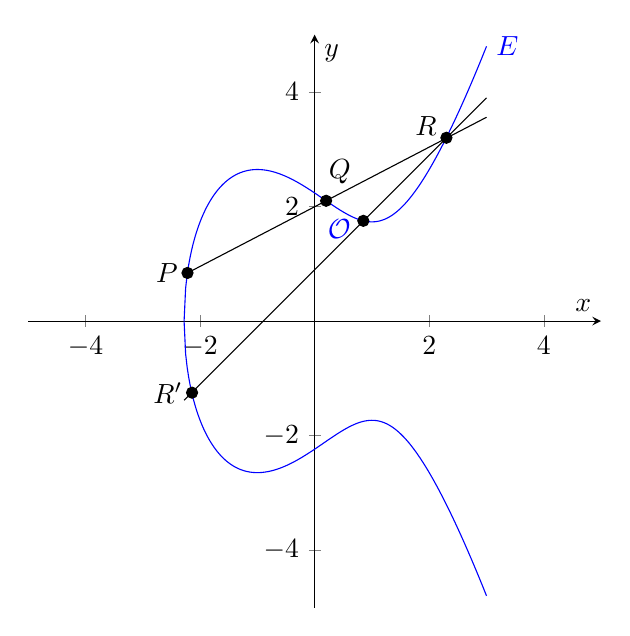
\begin{tikzpicture}

\begin{axis}[
xmin=-5,
xmax=5,
ymin=-5,
ymax=5,
xlabel={$x$},
ylabel={$y$},
scale only axis,
axis lines = middle,
domain=-2.2790178:3,
samples=201,
clip=false,
axis equal image=true
]
\addplot[blue] {sqrt(x^3-3*x+5)} node[right] {$E$};
\addplot[blue] {-sqrt(x^3-3*x+5)};
\addplot[black] { 4.83 / 2.42 + 1.26*x / 2.42};
\addplot[black] { 1.3 / 1.45 + x};


\draw[fill=black] (axis cs: -2.22, 0.84) circle (2pt) node [left] {$P$};
\draw[fill=black] (axis cs:  0.2, 2.1) circle (2pt);
\draw[color=black] (axis cs: 0.8, 2.6) node[left]{$Q$};
\draw[fill=black] (axis cs: 2.3, 3.2) circle (2pt);
\draw[color=black] (axis cs: 2.3, 3.4) node[left]{$R$};
\draw[fill=black] (axis cs: 0.85, 1.75) circle (2pt);
\draw[color=blue] (axis cs: 0.80, 1.6) node[left]{$\OO$};
\draw[fill=black] (axis cs: -2.14, -1.25) circle (2pt) node [left] {$R'$};
%\draw[color=black] (axis cs: -1.5, 2.7) node [left] {$P$};
\end{axis}
\end{tikzpicture}
\caption{Addisjon med baseelement $\OO$}
\end{figure}

\textbf{Skjæringspunkter}. La $C/K$ være en kurve som også er en varietet (tenk elliptisk kurve). Dersom vi tar to vilkårlige punkter $P, Q \in C$ får vi en unik linje, $L$, gjennom disse to punktene. Fra Bézouts teorem vet vi at denne linjen skjærer kurven i tre punkter. $L \circ C = \{P, Q, R \}$ for en $R \in C$. I spesialtilfellet der $P = Q$ setter vi linjen til å være tangentlinjen til $P$. Vi definerer nå avbildingen $\phi: C \times C \rightarrow C$ $(P, Q) \mapsto R$. Legg merke til at uansett hvilke to punkter du tar fra mengden av skjæringspunkter vil du alltid få den tredje. Dersom $L \circ C = \{P, Q, R\}$ vil $\phi(P, Q) = R$ og $\phi(P, R) = Q$ og $\phi(Q, R) = P$.

\begin{teorem}
En elliptisk kurve $E/K$ sammen med et baseelement $\OO \in E$ danner en abelsk gruppe under operasjonen $P + Q = \phi(\OO, \phi(P, Q))$, der $\phi$ er definert som over.

\begin{proof}
Vi må vise at $E$ er en gruppe og at den er abelsk, altså at den er assosiativ, har identitetselement, at alle punkter har en invers, og at den er kommutativ. La $P, Q, R \in E$, med $\OO$ som baseelement.
\begin{description}
\item[Assosiativitet] Skal vise at $(P + Q)+ R = P + (Q + R)$. La oss først definere noen punkter: $\phi(P,Q) = S'$, $\phi(\OO, S') = S$, $\phi(S, R) = T'$, $\phi(Q, R) = U'$, $\phi(\OO, U') = U$, $\phi(P, U) = T''$. Da har vi $(P + Q) + R) = \phi(\OO, T')$ og $P + (Q + R) = \phi(\OO, T'')$. Altså er det nok å vise at $T' = T''$.

Fra punktene over kan vi lage linjer som går gjennom punktene: $L_1: \{P, Q, S'\}$, $M_1: \{\OO, S', S\}$, $L_2: \{S, R, T' \}$, $M_2: \{ Q, R, U'\}$, $L_3: \{\OO, U', U \}$, $M_3: \{P, U, T''\}$ (Her er f.eks. $L_1$ linjen som går gjennom $P, Q, S'$ - det er der den skjærer $E$).

Vi kan nå sette sammen disse linjene ved enkel multiplikasjon. Husk at graden til hver linje er 1, så $L = L_1 * L_2 * L_3$ har grad 3 og er en kubisk kurve (ikke nødvendigvis irredusibel). Tilsvarende er $M = M_1 * M_2 * M_3$. 

La oss nå se på skjæringspunktene mellom disse linjene og kurven $E$. $E \circ L = \{P, Q, S', S, R, \OO, U', U, T' \}$, mens $E \circ M = \{\OO, S', S, Q, R, U', P, U, T'' \}$. Legg merke til at den eneste forskjellen er $T'$ og $T''$.

La oss nå lage en linje gjennom $T'$ som ikke går gjennom $T''$, Da har vi $N: \{T', W, W'\}$ for punkter $W, W' \in E$. Siden ingen av disse er i $M$ kan vi se på skjæringen mellom $N*M$ og $E$. $N*M \circ E = \{\OO, S', S, Q, R, U', P, U, T'', T', W, W'  \} = L \circ E \cup \{T'', W, W' \}$, altså finnes det en linje mellom $T'', W$ og $ W'$. Denne linjen må nødvendigvis være lik $N$ da den deler to punkter, så $T' = T''$ og vi har vist at operasjonen ar assosiativ. \cite[5.6.4]{fulton}

\item[Identitet] La $\phi(\OO, P) =R $, da har vi $P + \OO = \phi(\OO, \phi(P, \OO)) = \phi(\OO, R) = P$, samtidig er $\OO + P = \phi(\OO, \phi(P, \OO)) = \phi(\OO, R) = P$
\item[Invers] La $\phi(\OO, P) = R$, da har vi at $(P + \OO) + R = \OO + P + R = \OO + \OO = \phi(\OO, \phi(\OO, \OO))$. Annta $\{\OO, \OO, Q \}$ ligger på samme linje ($\phi(\OO, \OO) = Q$), da har vi $\phi(\OO, \phi(\OO, \OO)) = \phi(\OO, Q) = \OO$.
\item[Kommutativitet] Siden $\phi(P, Q) = \phi(Q,P)$ da dette bare er det tredje punktet på linjen har vi $P + Q = \phi(\OO, \phi(P, Q)) = \phi(\OO, \phi(Q,P)) = Q + P$
\end{description}
\end{proof}
\end{teorem}

Nå som vi vet at en elliptisk kurve danner en abelsk gruppe for et vilkårlig baseelement kan vi bestemme oss for et spesifikt. Det er vanlig å bruke punktet $[0,1,0]$ som baseelement/punkt i uendeligheten. Så videre i denne teksten anntar vi at $\OO = [0,1,0]$ da det forenkler en del regning. Legg merke til hvordan $\phi((x,y), \OO) = (x, -y)$ linjen mellom et punkt og $\OO$ blir den vertikale linjen.

Dette fører til at dersom $P = (x,y)$ vil $-P = \phi(P, \OO) = (x, -y)$.

Vi kommer til å bruke notasjonen $E(K)$ for å referere til de $K$-rasjonale punktene i $E$.

%$O = [0,1,0]$

%\subsection{Weierstrass form}
%\subsection{Invarianter}
%\subsection{Torsionundergrupper}
%Hva er dette, hvordan fungerer de.
%Hvorfor har vi $E[l]$ der $l$ deler $[E]$

%Hva er en supersingulær elliptisk kurve, finnes det alltid en slik?
%\subsection{genus}
%Når vi skal beskrive en elliptisk kurve trenger vi å vite hva en genus er. Intensjonen med dette kapitellet er å definere dette via divisorer av kurver. Om du allerede vet hva en genus er kan du fint hoppe over dette kapittelet.



\begin{teorem}(Riemann-Roch)
La $C/k$ være en glatt kurve med en kanonisk divisor $K_C$. Da finnes det ett heltall $g \geq 0$ slik at for alle divisorer $D \in Div(C)$, $$l(D) - l(K_C - D) = deg D - g + 1$$

\textbf{Bevis:} Se side 35. i \cite{silverman}
\end{teorem}
Merk: Dette teoremet kan forenkles til å kun basere seg på graden til kurven samt anntall singulære punkter når det er en kurve i planet.
\begin{definisjon}
heltallet $g$ fra teoremet over kalles \textbf{genus} til kurven $C$.
\end{definisjon}

\section{Avbildinger}
\subsection{Rasjonale avbildinger}
Vi skal nå begynne å se på avbildinger mellom varieteter og etter hvert elliptiske kurver. 


\begin{definisjon}
La $V/K$ være en varietet. Da er \textbf{koordinatringen} til $V$, $$K[V] = K[X_0, \ldots, X_n] / I(V)$$ altså restklassen av polynomer med $n$ variable modulo $I(V)$. 
\end{definisjon}

\begin{eksempel}
La $V/\FF_p$ være varieteten definert fra vår elliptiske kurvelikning $f(x,y)$. Da er koordinatringen på formen $\FF_p[x,y]/\langle y^2 - x^3 - ax - b \rangle$. Altså er f.eks $y^2$ det samme som $x^3 + ax + b$ i koordinatringen.
\end{eksempel} 

\begin{definisjon}
La $V/K$ være en affine varieteten definert av idealet $f(x,y)$. Da er \textbf{funksjonskroppen}, $K(V)$, kvotientkroppen til den tilhørende koordinatringen $K[V]$.
\end{definisjon}

\begin{definisjon}
La $V$ være en projektiv varietet definert av idealet $I = \langle f(X) \rangle$. Da er \textbf{funksjonskroppen}, $K(V)$, alle rasjonale funksjoner $g/h$ ($h \neq 0$) med følgende restriksjoner:
\begin{enumerate}[noitemsep]
    \item $g,h$ homogene polynomer i $K[x,y,z]$ av samme grad.
    \item $h$ er ikke i idealet $I(V)$
    \item $f_1/g_1$ og $f_2/g_2$ er ekvivalente dersom $f_1g_2 - f_2g_1 \in I(V)$
\end{enumerate}
\end{definisjon}
\textbf{TODO: vis at definisjonene er tilsvarende, og forklar hvorfor begge er med}


Vi er kun interessert i avbildinger mellom elliptiske kurver, vi kan derfor endre litt på måten vi skriver elementer i funksjonskroppen. Hver funksjon, $\phi$, er på formen $f(x,y)/g(x,y)$ for $f, g \in \overline{K}(E)$, altså i restklassen modulo idealet til et polynom på formen $y^2 - x^3 - Ax - B$. Dermed kan vi alltid erstatte $y^2$ med $x^3-Ax-B$, så vi får at leddet med $y$ maksimalt kan ha grad $1$. Dermed kan vi dele ut $y$, og vi får $f(x,y) = f_1(x) + f_2(x)y$ og $g(x,y) = g_1(x) + g_2(x)y$.  $$\phi = \frac{f_1(x) + f_2(x)y}{g_1(x) + g_2(x)y}$$ 
Men dette kan vi forkorte mer, vi kan multiplisere nevner og teller med $g_1(x) - g_2(x)y$ og så erstatte $y^2$ igjen, så vi sitter igjen med \begin{equation}
\label{forkortet funksjon}
phi = \frac{h_1(x) + h_2(x)y}{h_3(x)}
\end{equation}
Altså kan vi alltid skrive et element i funksjonskroppen til en elliptisk kurve på denne måten.

\begin{definisjon}
La $V_1$ og $V_2$ være varieteter i det projektive planet, og $f_0, f_1, f_2 \in \overline{K}(V_1)$.  Da er en \textbf{rasjonal avbilding} fra $V_1$ til $V_2$ en avbilding på formen $$ \phi: V_1 \rightarrow V_2 \text{, } \phi = [f_0, f_1, f_2] $$ 
Der man evaluerer $\phi$ komponentvis, altså $\phi(P) = [f_0(P), f_1(P), f_2(P)]$ for alle $P \in V_1$ der $f_0, f_1 og f_2$ er definert og $P \neq 0$.
\end{definisjon}

På samme måte som i seksjon 2 kan vi tenke på dette som affine varieteter mens vi i realiteten bruker projektive varieteter. Altså blir en rasjonal avbilding på formen $\phi: V_1 \rightarrow V_2, (x,y) \mapsto (f(x,y), g(x,y))$ i stedet for slik den er definert over.


\begin{definisjon}
La $\phi$ være en rasjonal avbilding. Vi sier at $\phi$ er \textbf{definert} i et punkt $P \in V_1$ dersom det finnes et funksjon $g \in \overline{K}(V_1)$ slik at
\begin{enumerate}[noitemsep]
    \item $g f_i$ er definert i punktet $P$
    \item $(gf_i)(P) \neq 0$ for minst én $i$
\end{enumerate}
Vi skriver så $$ \phi(P) = [(gf_0)(P), \ldots, (gf_n)(P)] $$
\end{definisjon}

\begin{definisjon}
La $\phi: V_1 \rightarrow V_2$ være en rasjonal avbilding. Vi sier at $\phi$ er en \textbf{morfisme} hvis den er definert i alle punkt $P \in V_1$.
\end{definisjon}

Vi kommer ikke til å være opptatt av å skille morfier fra rasjonale avbildinger da vi automatisk får slike morfier når vi ser på avbildinger fra en glatt projektiv kurve til en varietet, men vi må kjenne til begrepet for å vise at dette stemmer.

\begin{teorem}
Dersom $C/K$ er en glatt projektiv kurve vil alle rasjonelle avbildinger fra $C/K$ til en projektiv varietet $V/K$ være morfier.

\begin{proof}
For å bevise dette må vi introdusere mange ting... \textbf{TODO: Prøv å fjerne ting som ikke er viktig}

La først $M_P = \{f \in \overline{K}(C) \mid f(P) = 0\}$

Så definerer vi ordenen til $f \in \overline{K}[C]$, $ord_P(f) = sup\{d \in \ZZ \mid f \in M_P^d\}$, det er lett å sjekke at $ord_P(f/g) = ord_P(f) - ord_P(g)$

La nå $t \in \overline{K}[C]$ være slik at $ord_P(t) = 1$ (dette kalles "Uniformizer")

La $\phi = [\phi_0, \ldots, \phi_n]$ være en vilkårlig rasjonal avbilding fra $C/K$ til $V/K$. $\phi$ er da definert i punktet $P$ hvis og bare hvis $ord_P(\phi_i) \geq 0$ for minst én $i$. \textbf{TODO: Bevis for dette - definisjon kan da ikke være nok}.

La oss nå se på alle ordenene til $\phi_i$, merk at hver funksjon er på formen $f_i/g_i \in \overline{K}(V)$, da er $ord_P(\phi_i) = ord_P(f_i) - ord_P(g_i)$, så denne kan potensielt være negativt og dermed udefinert i punktet $P$. Heldigvis kan vi multiplisere med en funksjon fra $\overline{K}(V)$, så la $n = min\{ord_P(\phi_i)\}$ da vil $ord_P(t^{-n}) = -n$ (Dette følger fra teoeremet innenfor diskre valueringsring). Hvis vi nå ser på $[t^{-n}\phi_0, \ldots, t^{-n}\phi_n]$ har vi at $ord_P(t^{-n}\phi_i) \geq 0$ for alle $i$, og $ord_p(t^{-n}\phi_j) = 0$ for minst én $j$. Altså er $\phi$ definert i punktet $P$, og tilsvarende kan gjøres for alle $P$ i $C/K$, så $\phi$ er en morfi.


\textbf{TODO: Dersom dette skal vises ordentlig må jeg gå om "Diskre valueringsring - "discrete valuation ring" og finne en bedre forklaring}
\end{proof}
\end{teorem}

\begin{teorem}
\label{morfi konstant eller surjektiv}
La $\phi: E_1 \rightarrow E_2$ være en morfi mellom to elliptisk kurver. Da er enten $\phi$ konstant eller surjektiv. \textbf{MERKNAD: Vanligvis fra morfi mellom to "kurver" - ikke nødvendigvis elliptiske kurver}
\textbf{TODO: Finn ut, og bevis dette}
Bevis:
Se [243, I \$5, theorem 4]
\begin{proof}
Først annta $E_1$ defineres av $y^2 - x^3 - Ax - B$, og $E_2$ defineres av $y^2 - x^3 - A'x - B'$ for $A, B, A', B' \in K$.
Vi vet fra \ref{forkortet funksjon} at $\phi = (\frac{h_1(x) + h_2(x)y}{h_3(x)}, \frac{g_1(x) + g_2(x)y}{g_3(x)}$. La så $P = (a,b) \in E_2$. 

Se på funksjonen $f(x) = h_1(x) + h_2(x)y - a h_3(x)$. $f$ kan da være konstant eller ikke.
Annta $f$ er ikke-konstant. Da vil $f$ ha en rot, $x_0$ i $\overline{K}$, altså er $f(x_0) = 0$, og vi får $\frac{h_1(x_0) + h_2(x_0)y}{h_3(x_0)} = a$. Bruk så denne roten, $x_0$, og sett $y_0 = \sqrt{x_0^3 + Ax_0 + B}$. Da vet vi at $\phi$ er definert for $(x_0, y_0) \in E_1$, og  $\phi(x_0, y_0) = (a, b')$ der $b = a^3 + A'a+B = b'$. Siden både $(a, b)$ og $(a,-b) = (a, b')$ er punkter i $E_2$ må vi vite at de begge har et prebilde. Dersom $b' = -b$ har vi også at $(x_0, -y_0) \in E_1$ og $\phi(x_o, -y_0) = (a, -b') = (a,b)$. Altså vil alle punkter i $E_2$ ha et prebilde i $E_1$.

Annta så at $f$ er konstant. \textbf{Her stemmer det ikke helt}

\cite[II 2.1]{silverman}
\end{proof}
\end{teorem}

\begin{definisjon}
Vi sier at to varieteter er isomorfe dersom det finnes en mrfi $\phi: V_1 \rightarrow V_2$ og en morfi $\psi: V_2 \rightarrow V_1$ slik at $\phi \circ \psi$ og $\psi \circ \phi$ er identitetsavbildinger på $V_2$ og $V_1$. 
\end{definisjon}

\textbf{TODO: Ikke-trivielt eksempel to isomorfe elliptiske kurver}

\subsection{Isogenier}
Isogenier er sentralt for protokollen vi skal studere. 

Selve definisjonen av en isogeni kommer fra at vi ønsker oss en avbilding som bevarer strukturen til den elliptiske kurven som en varietet, og som en abelsk gruppe. Det finnes flere tilsvarende definisjorer, men vi kommer til å ta utgangspunkt i følgende.
\begin{definisjon}
La $E/K$ være en elliptisk kurve. Vi sier at en \textbf{isogeni}, $\phi$, er en morfi, $\phi: E \rightarrow E'$, som også tilfredsstiller $\phi(\OO_E) = \OO_{E'}$
\end{definisjon}

Legg merke til at $\phi: E \rightarrow \{\OO \}$ tilfredsstiller kravene til en isogeni. Dette kalles konstantavbildingen og er i praksis en ubrukelig isogeni. Derfor kommer vi framover til å anta at $\phi$ er ikke-konstant.

Nå som vi vet hva en isogeni er kan vi videre forkorte (\ref{forkortet funksjon}) slik at den tar hensyn til bevaring av gruppeoperasjonene. La $\phi = (\frac{f_1(x) + f_2(x)y}{f_3(x)}, \frac{g_1(x) + g_2(x)y}{g_3(x)})$. Siden $\phi(-P) = -\phi(P)$ for $P = (a,b) \in E/k$ har vi at $\frac{f_1(a) + f_2(a)(-b)}{f_3(a)} = \frac{f_1(a) + f_2(a)b}{f_3(a)}$, altså får vi $\frac{f_1(x) + f_2(x)y}{f_3(x)} = \frac{f_1(x)}{f_2(x)}$. Tilsvarende for $b$ har vi $\frac{g_1(a) + g_2(a)(-b)}{g_3(b)} = -\frac{g_1(a) + g_2(a)b}{g_3(a)}$, altså må $\frac{g_1(a) - g_2(a)b}{g_3(a)} = \frac{g_2(a)y}{g_3(a)}$. Med andre ord kan vi alltid skrive en isogeni på formen 
\begin{equation}
\label{forenklet isogeni}
\phi = (\frac{u(x)}{v(x)}, \frac{s(x)}{t(x)}y)
\end{equation}

\begin{definisjon}
La $\phi$ være en isogeni på den forenklede formen (\ref{forenklet isogeni}). Vi sier at \textbf{graden} til isogenien, $deg(\phi)$ er den største graden blant $u$ og $v$, altså $$deg(\phi) = max \{deg(u), deg(v) \} $$
\end{definisjon}

\begin{definisjon}
La $\phi: E_1 \rightarrow E_2$ være en isogeni, der $\OO \in E_2$  er baseelementet til $E_2$. Vi sier at \textbf{kjernen}, $ker(\phi) = \{P \in E_2 \mid \phi(P) = \OO\}$
\end{definisjon}

\begin{teorem}
\label{unik_kjerne}
La $E$ være en elliptisk kurve og $\Phi$ være en endelig underrguppe av $E(K)$, da er det en unik elliptisk kurve $E'$ og en separabel isogeni $\phi$ der $\phi: E \rightarrow E'$ slik at $ker(\phi) = \Phi$

\cite[6.10]{sutherland-notes}
\end{teorem}

En viktig egenskap ved isogenier er at de kan dekomponeres i isogenier av lavere grad. Dette er særdeles gunstig da mengden arbeidskraft nødvendig er proposjonal med graden til isogenien.

\begin{korollar}
\label{isogeni_dekomponering}
La $\phi: E_1 \rightarrow E_2$ være en isogeni av sammensatt orden $n$. En slik isogeni kan alltid dekomponeres til en "sekvens" av mindre isogenier av primtallsorden.

\begin{proof}
La $G = ker(\phi)$. Siden $G$ er en abelsk gruppe vet vi at den inneholder en undergruppe, $H \leq G$, av orden $p$ der $p$ er et primtall. Av teorem \ref{unik_kjerne} har vi at det finnes en isogeni $\phi_1: E_1 \rightarrow E_3$ der $ker(\phi_2) = H$. Videre vet vi at $\phi_1(G) \cong G/H$ (siden $\phi_1$ har kjerne $H$ og $\phi_1(G) \subset E_3(\overline{K})$). Med dette kan vi lage en til isogeni, $\phi_2 : E_3 \rightarrow E_4$ med kjerne $ker(\phi_2) = G/H$. Sammensetningen, $\phi_2 \circ \phi_1: E_1 \rightarrow E_4$ er nå en isogeni med $ker(\phi_2 \circ \phi_1) = G/H \times H = G = ker(\phi)$, altså er $E_4$ og $E_2$ isomorfe. Med andre ord finnes det en isogeni av grad 1, $i: E_4 \rightarrow E_2$. Altså har vi $\phi = i \circ \phi_2 \circ \phi_1$, der $\phi_1$ har grad $p$, graden til $\phi_2$ er $n/p$, og graden til $i$ er 1. Dermed kan vi fortsette med $\phi_2$ til vi kun har primtall.

\begin{figure}[h!]
    \centering
\begin{tikzcd}
E_1 \arrow{r}{\phi_1} \arrow[dashed, bend right]{rrr}[description]{i \circ \phi_2 \circ \phi_1} & E_3 \arrow{r}{\phi_2} & E_4 \arrow{r}{i} & E_2
\end{tikzcd}
\end{figure}
\end{proof}
\end{korollar}

\begin{eksempel}
\label{eksempel_dekomponere_isogeni}
La $E/\FF_q$ være en elliptisk kurve, og $\langle R\rangle \leq E(\FF_q)$, der $|\langle R \rangle | = p^e$. Vi ønsker å lage en isogeni, $\phi$, fra $E$ med kjerne $\langle R \rangle$. Ved hjelp av korollar \ref{isogeni_dekomponering} har vi at $\phi = i \circ \phi_e \circ \ldots \circ \phi_1$. Der $i$ er en isomorfiavbilding. Siden vi her ikke er ute etter den spesifikke elliptiske kurven, men heller bare én vilkårlig, kan vi droppe isomorfiavbildingen.

Når vi skal beregne isogeniene $\phi_i$ gjør vi dette iterativt, og starter med $\phi_1$. Denne skal ha kjerne av grad $p$, noe vi får ved å regne ut $langle p^{e-1}R \rangle$. Altså blir $\phi_1 : E \rightarrow E/\langle p^{e-1}R \rangle = E_1$. Når vi skal beregne videre vil vi ikke nødvendigvis ha punktet $R \in E_1$, derfor må vi flytte det over med $R_1 := \phi_1(R)$. Merk at dette punktet har orden $p^{e-1}$ siden $\phi_1$ er en gruppehomomorfi med kjerne $p$. Dermed kan vi lage neste isogeni, $\phi_2 : E_1 \rightarrow E_1 / \langle p^{e-2}R_1 \rangle = E_2$. Dette kan vi fortsette med helt til vi får $\phi_e : E_{e-1} \rightarrow E_{e-1} /langle R_{e-1} \langle$. 

Når vi setter dette sammen igjen får vi $$\phi = \phi_e \circ \phi_{e-1} \circ \ldots \circ \phi_1 $$ Av med kjerne $ker(\phi) \cong (\ZZ_p)^e$, altså vil graden til $\phi$ være $p^e$.
\end{eksempel}

Men vi er ikke bare interessert i den abstrakte teorien, vi er også interessert i hvordan vi kan bruke dette. Derfor introduserer vi nå noen algoritmer fra for å beregne isogenier ut fra kjernen. Merk at dette ikke nødvendigvis er de raskeste formlene for å beregne isogenier, men de er relativt enkle, og gir en god nok innføring for vår del.


Først tar vi algoritmen for å beregne isogenier av grad 2
\begin{teorem}
(Vélu) \cite{velu} La $E_1/K$ være en elliptisk kurve definert av $y^2 - x^3 - Ax - B$. La så $x_0$ være en rot av $x^3 + Ax + B \in \overline{K}[x]$. Sett så $t = 3x_0^2 + A$ og $w = x_0 + t$. Den rasjonale avbildingen $$\phi(x,y) = \Bigg( \frac{x^2-x_0x+t}{x-x_0}, \frac{(x- x_0)^2 - t}{(x-x_0)^2}y \Bigg)$$ er en separabel isogeni fra $E_1$  til $E_2$, der $E_2$ er den elliptiske kurven definert av $y^2 - x^3 - A'X - B$ der $A' = A - 5t$ og $B' = b - 7w$. Kjernen til $\phi$ er gruppen av orden 2 som genereres av $(x_0, 0)$. 
\begin{proof}
Se \cite[6.12]{sutherland-notes}
\end{proof}
\end{teorem}

Så har vi isogenier av odde grad. 
\begin{teorem}
(Vélu) \cite{velu} La $E_1/K$ være en elliptisk kurve definert av  $y^2 - x^3 - Ax - B$. La så $G$ være en endelig undergruppe av $E(\overline{K})$ av oddetallsorden. For hver ikke-null $Q = (x_Q, y_Q) \in G$ definerer vi $t_Q = 3x_Q^2 + A$, $u_Q = 2y_Q^2$ og $w_Q = u_Q + t_Qx_Q$. Videre setter vi $t = \sum t_Q$, $w = \sum w_Q$ og $$r(x) = x + \sum (\frac{t_Q}{x - x_Q} + \frac{u_Q}{(x - x_Q)^2})$$. Da vil den rasjonale avbildingen $$ \phi(x,y) = (r(x), r'(x)y)$$ være en separabel isogeni fra $E_1$ til $E_2$ der $E_2$ er definer av $y^2 - x^3 - A'x - B' $ med $A' = A - 5t$ og $B' = B - 7w$ med kjerne $ker(\phi) = G$

\begin{proof}
Se \cite[6.14]{sutherland-notes}
\end{proof}
\end{teorem}



\begin{eksempel}
La $E/\FF_{11}$, $E: y^2 = x^3 + 5$. Her vil $E(\FF_{11})= \{\OO, (0,4),$ $(0,7), (4,5), (4,6), (5,3),$ $(5,8),$ $(6,1),$ $(6,10),$ $(8,0),$ $(10,2),$ $(10,9) \}$. Vi kan enkelt sjekke at $(0,4)$ og $(0,7)$ har orden $3$. Altså med $G = \{\OO, (0,4), (0,7)\}$ har vi en endelig undergruppe med orden $3$. La oss nå regne ut isogenien med kjerne $G$.

Ikke-null $Q \in G$ er da $(0,4)$ og $(0,7)$. $A = 0, B = 5$

$t_1 = 3*0^2 + 0 = 0$, $t_2 = 3*0^2 + 0$, altså blir $t = t_1 + t_2 = 0$.

$u_1 = 2*4^2 = 10$, $u_2 = 2*7^2 = 10$, siden $t = 0$ blir $w_1 = u_1$ og $w_2 = u_2$. altså blir $w = 9$.

$r(x) = x + \frac{10}{x^2} + \frac{10}{x^2} = \frac{x^3 + 9}{x^2}$

$A' = 0, B' = 5 - 7*9 = 8$

Altså blir $$\phi(x,y) = \Big(\frac{x^3 + 9}{x^2}, \frac{3x^3y + 4y}{x^3}\Big)$$ en isogeni fra $E$ til $E_2: y^2 - x^3 - 8$. 

Vi kan finne ut at $E_2(\FF_{11} = \{\OO, (0,1),$ $(1,3), (1,8),$ $(2,4), (2,7),$ $(5,1), (5,10),$ $(6,2), (6,9),$ $(8,5), (8,6),$ $(9,0)\}$. 

En interessant observasjon vi kan se er at alle $\FF_{11}$-rasjonale punkter i $E_2$ som også har $\FF_{11}$-rasjonalt prebilde har tre slike prebilder i $E$, for eksempel $\phi(0,4) = (0,1) = \phi(0,7) = \phi(0, 1)$, og tilsvarende $(8,6) = \phi(4,5) = \phi(5,3) = \phi(10,9)$. Men begge kurvene har like mange punkter. f.eks. er $(1,3)$ et slikt punkt som blant annet har prebildet $(x,y)$\textbf{Todo: Finn dette punktet/prebildet}



\textbf{TODO: Tegn opp grafer fra $E_1$ til $E_2$, se på hvilke hvor de nye punktene kommer fra}

\end{eksempel}

Nå som vi kan beregne isogenier av grad 2 og odde grad, har vi mulitheten til å sette disse sammen til en isogeni av vilkårlig grad.


\subsection{Endomorfier}

\begin{definisjon}
La $E/K$ være en elliptisk kurve. Vi sier at en isogeni $\phi$ er en \textbf{endormorfi }dersom den avbilder $E$ på seg selv, altså $\phi: E \rightarrow E$.

Dersom den i tillegg er isomorfisk sier vi at det er en \textbf{automorfi}.
\end{definisjon}



\textbf{TODO: Eksempel delvis tatt fra Washington, se om det bør fjernes/erstattes}
\begin{eksempel}
\label{enkel_endormorfi}
La $E$ være den elliptiske kurven gitt av $f(x,y) = y^2 - x^3 - B$. Da vil $\alpha(P) = [2]P$ være en endomorfi gitt av $\alpha(x,y) = (f_1(x,y), f_2(x,y))$, der 
\begin{align*}
f_1(x,y) &= \Big(\frac{3x^2}{2y} \Big)^2 - 2x & f_2(x,y) &= \frac{3x^2}{2y}\bigg(\Big(\frac{3x^2}{2y} \Big)^2 - 3x\bigg) - y 
\end{align*}
\end{eksempel}

En spesielt interessant endomorfi er \textbf{Frobenius endomorfien}. La $\phi_q : \overline{\FF_q} \rightarrow \overline{\FF_q}$, slik at $x \mapsto x^q$. Da er frobenius enomorfien $\pi_q: E \rightarrow E$, med $(x,y) \mapsto (x^q, y^q)$

\begin{lemma}
La $E/\FF_q$, og $(x,y) \in E(\overline{\FF_q})$, da har vi \begin{enumerate}
\item $\pi_q(x,y) \in E(\overline{\FF_q})$
\item $(x,y) \in E(\FF_q)$ hvis og bare hvis $\pi(x,y) = (x,y)$
\end{enumerate}

\begin{proof}
Se \cite[93, 4.5]{washington}
\end{proof}
\end{lemma}


\section{Struktur}


\label{Elementer i elliptisk kurve}

\begin{teorem}
La $q = p^2$, der $p$ er et primtall, og $\FF_q$ være en endelig kropp, og $E/\FF_q$ en supersingulær elliptisk kurve. Da har vi $\#E(\FF_q) = (p \mp 1)^2$

\begin{proof}
Fra \cite{elements_elliptic_curve} har vi at $\#E(\FF_q) = 1 + q - \beta$ der $\beta = \pm 2 \sqrt{q}$, altså er $\beta = \pm p$. Da har vi $E(\FF_q) = 1 + p^2 \mp p = (p-1)^2$
\end{proof} 
\textbf{TODO: Bedre bevis for dette, hvorfor må $E$ være supersingulær?}
\end{teorem}

Nå vet vi at $E(\FF_q)$ er en abelsk gruppe med $(p \mp 1)^2$ punkter. Altså kan vi si noe om strukturen.

\begin{eksempel}
La $l_A$ og $l_B$ være to (små) primtall, $e_A, e_B$ og $f \in \ZZ^+$ være positive heltall slik at $p = l_A^{e_A}l_B^{e_B}f \pm 1$ er et primtall. Da er $\FF_q = \FF_{p^2}$ en endelig kropp. La så $\#E(\FF_q) = (p \mp 1)^2 = (l_A^{e_A}l_B^{e_B}f)^2$. Da har vi fra Teorem \ref{finite abelian group} at $E(\FF_q) \cong \ZZ/(l_A^{e_A}l_B^{e_B}f)\ZZ \times \ZZ/(l_A^{e_A}l_B^{e_B}f)\ZZ$
\end{eksempel}

Siden vi vet at $E/\FF_p$ danner en endeliggenerert abelsk gruppe har vi fra teorem \ref{fundamentalteoremet} at denne kan dekomponeres til et direktesum av sykliske undergrupper. Altså finnes det undergrupper til den elliptiske kurven. 

En interessant problemstilling er hvorvidt en restklasse til en elliptisk kurve også danner en elliptisk kurve.


Skal vise:
$E/\Phi$ er også en elliptisk kurve

Oppgave 3.13

Undegrupper

\subsection{J-invariant}

I protokollen vi skal undersøke senere er vi interessert i å komme fram til samme verdi når vi har to potensielt ulike isomorfe elliptiske kurver. Derfor er det nyttig å finne en invariant over isomorfiavbildinger. 

\begin{definisjon}
La $E/K$ være en elliptisk kurve på formen $y^2 = x^3 + Ax + B$. Vi sier at \textbf{diskriminanten}, $\Delta$, er definert som $$ \Delta = -16(4A^3 + 27B^2) $$
\end{definisjon}
Merk, diskriminanten sier noe om hvorvidt en kurve er singulær eller ikke. Når $\Delta \neq 0$ har vi at kurven er ikkesingulær, og altså en elliptisk kurve.

\begin{definisjon}
La $E/K$ være en elliptisk kurve på formen $y^2 = x^3 + Ax + B$. Vi sier at \textbf{j-invarianten}, j, er definert som $$ j = -12^3 \frac{(4A)^3}{\Delta} $$
\end{definisjon}

\begin{proposisjon}
To elliptiske kurver er isomorfe hvis og bare hvis avbildingen er på formen $[u^2x, u^3y]$ der $u \in \overline{K}$. (gjelder kun med karakteristikk $\notin \{2,3 \}$) \textbf{TODO: Bevis dette}
\end{proposisjon}

\begin{proposisjon}
To elliptiske kurver er isomorfe over $\overline{K}$ hvis og bare hvis de har samme j-invariant.

\begin{proof}
La $E_1/K$ og $E_2/K$ være elliptiske kurver på formen $y^2 = x^3 + ax + b$ og $y^2 = x^3 + \alpha x + \beta$ slik at $\phi: E_1 \rightarrow E_2$ er en isomorfi. Da har vi  at $\phi(x) = u^2x$ og $\phi(y) = u^3y$, eller med enkel substitusjon: 
\begin{equation*}
    a = u^4 \alpha \text{ og } b = u^6 \beta 
\end{equation*}
"$\Leftarrow$": La begge kurvene $E_1$ og $E_2$ ha samme j-invariant, $j$. Da har vi tre tilfeller vi må ta hensyn til:
\begin{description}
\item[j = 0]: Da har vi fra definisjonen av $j$-invariant at $a = \alpha = 0$. Da blir også $b \neq 0$ og $\beta \neq 0$ siden $\Delta \neq 0$ for elliiptiske kurver. Må vise at $b = u^6 \beta$, altså at $\frac{b}{\beta}$ har en sjetterot i $\overline{K}$ \textbf{Hvordan vet vi dette?}

\item [j = 12$^3$]: Fra definisjonen av $j$, må 
\begin{equation*}
    \frac{(4a)^3}{-16(4a^3+27b^2)} = -1
\end{equation*}
så $a \neq 0$, noe som medfører at $b = 0$. (Tilsvarende for $\alpha$ og $\beta$. Da har vi at $a = u^4\alpha$, eller $u = \sqrt[4]{\frac{a}{\alpha}}$

\item[Resten] Siden hverken $a, b, \alpha$, eller $\beta = 0$ (dersom en av de var det ville j-invarianten vært $0$ eller $12^3$, dersom begge var det blir $\Delta = 0$) har vi at $u = \sqrt[4]{\frac{a}{\alpha}} = \sqrt[6]{\frac{b}{\beta}}$
\end{description}
"$\Rightarrow$" \textbf{Må bevise dette}
\end{proof}
\end{proposisjon}

Konsekvensen av denne "hvis og bare hvis" proposisjonen er at vi har en invariant over isomorfe elliptiske kurver, og denne er unik.

\subsection{Torsiongrupper}

Torsiongrupper er en viktig del av protokollen vi senere skal se på. Vi kommer til å bruke de til å lage kjerner av riktig størrelse og må vite litt om hvordan de ser ut.

\begin{definisjon}
La $E$ være en elliptisk kurve, og $m$ et heltall. Vi sier at multiplikasjon av $m$-avbildingen, $[m]: E \rightarrow E$ er definert som $[m]: P \mapsto \underbrace{P + \ldots, + P}_{m \text{ ganger}}$
\end{definisjon}

\begin{definisjon}
La $E$ være en elliptisk kurve, og $m$ være et heltall. Vi sier at $m$-torsiongruppa, $E[m]$ er alle punktene som multiplisert med $m$ blir $\OO$: $$E[m] = \{P \in E \mid [m]P = \OO \} $$
\end{definisjon}

Merk, en torsongruppe inneholder ikke bare alle punktene av orden $m$. F.eks. vil $E[4]$ også inneholde punkter av orden 2 da $[4]P = [2][2]P = [2] \OO = \OO$.

\begin{proposisjon}
La $E$ være en elliptisk kurve, og $m$ et heltall. Da er $deg[m] = m^2$. 

\begin{proof}
\textbf{TODO: Bevis dette} 
\end{proof}
\end{proposisjon}

\begin{korollar}
\label{torsonstruktur}
La $E$ være en elliptisk kurve, $m$ være et positivt heltall og $p = char(K)$. Da har vi følgende:
\begin{enumerate}
    \item Hvis $p = 0$ eller $p \nmid m$ da er $$ E[m] \cong \frac{\ZZ}{m\ZZ} \times \frac{\ZZ}{m\ZZ} $$
    \item Ellers er en av følgende riktige \begin{enumerate}
        \item $E[p^e] = \{O\}$ for alle $e = 1, 2, 3, \ldots$
        \item $E[p^e] \cong \frac{\ZZ}{p^e\ZZ}$ for alle $e = 1, 2, 3, \ldots$
    \end{enumerate}
\end{enumerate}

\begin{proof}
\cite[III 6.4]{silverman}
\end{proof}
\end{korollar}

\begin{eksempel}
La $E/\FF_q$ være en elliptisk kurve med orden $( l_A^{e_A} l_B^{e_B}f) ^2$. der $l_A$, $l_B$, og $\sqrt(q)$ er (ulike) primtall. Siden $q \nmid l_A^{e_A}$ har vi at torsongruppa $$E[l_A^{e_A}] \cong \frac{\ZZ}{l_A^{e_A} \ZZ} \times \frac{\ZZ}{l_A^{e_A} \ZZ}$$. Altså vil to lineært uavhengige punkter $P, Q \in E$ generere hele torsongruppa. 
\end{eksempel}


\begin{proposisjon}
\label{torson_generatorer}
La $E/\FF_q$ være en elliptisk kurve og $E[p^e]$ være en torsongruppe der $p$ er et primtall og $char(\FF_q) \nmid p$. Da vil $E[p^e]$ ha $(p^e - p^{e-1})^2$ elementer av orden $p^e$. 

\begin{proof}
Siden $p$ er primtall vil $\ZZ / p^e\ZZ$ være en syklisk gruppe (av Gauss). Antall generatorer i denne gruppa vil være $\phi(p^e) = p^e - p^{e-1}$ (Eulers phi-funksjon). Siden $E[p^e] = \ZZ / p^e\ZZ \times \ZZ / p^e\ZZ$ finnes det $(p^e - p^{e-1})^2$ elementer av orden $p^e$
\end{proof}
\end{proposisjon}

\begin{eksempel}
\label{torson_automorfi}
La $E/\FF_q$ være en elliptisk kurve der $\#E(\FF_q) = (l_A^{e_A})^2H$ der $l_A^{e_A} \nmid H$ 

Siden vi vet at $E$ er en abelsk gruppe har vi at $E(\FF_q) \cong \frac{\ZZ}{l_A^{e_A} \ZZ}^2 \oplus C_H$, der $C_H$ er en syklisk gruppe av orden $H$. Vi kan nå se på avbildingen $[H]$. Denne fungerer som en automorfi på på $E[l_A^{e_A}]$ fordi $l_A \nmid H$. I tillegg vil det sende alle elementer i $C_H$ til $e$. Altså blir det en avbilding på formen $[H]: E \rightarrow  \frac{\ZZ}{l_A^{e_A} \ZZ} \times \frac{\ZZ}{l_A^{e_A} \ZZ}$. 

Vi kan med andre ord bruke dette for å finne et element som ligger i torsongruppa $E[l_A^{e_A}]$.
\end{eksempel}



\textbf{TODO: Skriv om lineart uavhengige punkter som generer torsongruppa, tegn bilde (gitter-aktig)}

\subsection{Strukturen til $E$}

\begin{teorem}
\textbf{Mordell–Weil} La $K$ være en endelig kropp. Da vil de $K$-rasjonale punktene til en elliptisk kurve danne en endeliggenerert abelsk gruppe.
\begin{proof}
For bevis, se \cite[207, VIII]{silverman}
\end{proof}
\end{teorem}

Vi vet nå at $E/K$ danner en endeliggenerert abelsk gruppe dersom $K$ er endelig.
Vi er ofte interessert i kardinaliteten, antall elementer, til en elliptisk kurve - vi bruker den 
korte notasjonen $\#E(K)$ for å indikere antall $K$-rasjonale punkter i $E$.

\begin{teorem}
La $E/\FF_q$ være en ellliptisk kurve. Da vil enten 
\begin{align*}
E(\FF_q) \cong \ZZ/n\ZZ & \text{ eller } & E(\FF_q) \cong \ZZ/n\ZZ \oplus \ZZ/n\ZZ & 
\end{align*}
\begin{proof}
fra teorem \ref{finite abelian group} har vi at $E(\FF_q)$ er isomorf til en direktesum av sykliske grupper, $\ZZ/n_1\ZZ \oplus \ldots \oplus \ZZ/n_r\ZZ$. Med $n_i \mid n_{i+1}$. For hver $i$ vil gruppen $\ZZ/n_i\ZZ$ ha $n_i$ elementer av orden som deler $n_i$. Dette medfører at $E(\FF_q)$ har $n_1^r$ elementer av orden $n_1$. Men fra teorem \ref{torsonstruktur} har vi at det maksimalt er $n_1^2$ slike. Altså må $r \leq 2$. \cite[91, Teorem 4.1]{washington}
\end{proof}
\end{teorem}

\begin{teorem}
(Hasse) \textbf{TODO: Finn riktig referanse til Hasses opprinnelige teorem}. La $E/\FF_q$. Da vil ordenen til $F_1$ tilfredsstille $$| q + 1 - \#E(\FF_q) | \leq 2 \sqrt{q}$$
\end{teorem}

\textbf{TODO: Bruk hasses teorem til å sette begrensingen, vis så for elliptiske kurver at det finnes en kurve som er definert som den under.}


\subsection{Supersingulære kurver}

\begin{definisjon}
La $E/K$ være en elliptisk kurve definert over en kropp $K$ med karakteristikk $p$. Vi sier at $E$ er \textbf{supersingulær} dersom det eneste punktet i $E[p] = \{\OO \}$
\end{definisjon}

\begin{proposisjon}
La $E$ være en elliptisk kurve over $\FF_{p^n}$ der $p$ er et primtall og $n$ er et positivt heltall. La så $a = p^n + 1 - \# E(\FF_{p^n})$. Da er $E$ supersingulær hvis og bare hvis $a \cong 0 \mod{p}$, eller tilsvarende $\#E(\FF_{p^n}) \cong 1 \mod{p}$.
\end{proposisjon}

\begin{proposisjon}
La $q = p^n$ for et primtall $p$ og positivt heltall $n$ og $B \in \FF_q^x$, der $q \cong 2 \mod{3}$. Da vil den ellitpsike kurven gitt av polynomet $y^2 - x^3 - B$ være supersingulær.

\begin{proof}
La $\psi:  \FF_q^x \rightarrow  \FF_q^x$ være homomorfien definert av $\psi(x) = x^3$. Siden $q-1$ ikke er en multippel av $3$ er det ingen elementer av orden $3$ i $ \FF_q^x$, altså er $ker(\psi) = \{0\}$. Med andre ord, $\psi$ er injektiv. Siden det er en avbilding fra en endelig gruppe til seg selv er den altså også surjektiv. Noe som betyr at alle elementer i $\FF_q$ har en unik tredjerot i $\FF_q$ (Merk at $\FF_q^x = \FF_q \setminus \{0\}$, og $0 = 0^3$. Spessielt har alle punkter, $y^2 - B$, en tredjerot, $x$ som gir oss $y^2 - x^3 - B = 0$ - altså har vi $q$ punkter. Dersom vi legger til punktet i uendeligheten, $\OO$ har vi $q+1$ punkter, og $E$ er supersingulær.\textbf{TODO: sjekk dette,Korollar 3:30 sier at dette gjelder dersom $q$ er primtall, ikke ellers.}
\cite[4.3.1]{washington}
\end{proof}
\end{proposisjon}

\section{Protokoller}
\subsection{SIDH}
Supersingular Isogeny-based Diffie Hellman (eller bare SIDH) er et kroptosystem som inkluderer zero-knowledge, nøkkelutveksling og offentlig-nøkkel kryptering. Denne seksjonen er hentet fra \cite{sidh}
\subsubsection{Nøkkelutveksling}
\begin{figure}[h!]
    \centering
      \begin{tikzcd}
        E_0 \arrow{r}{\phi_A} \arrow[swap]{d}{\phi_B} & E_A \arrow{d}{\phi_{AB}} \\
         E_B \arrow{r}{\phi_{BA}}& E_{AB} \cong E_{BA}
      \end{tikzcd}
    \caption{Isogenidiagram}
    \label{fig:my_label}
\end{figure}
\textbf{Oppsett}: Velg en en supersingulær elliptisk kurve $E_0$ definert over $\FF_p^2$, der $p = l_A^{e_A}l_B^{e_B}f \pm 1 $. Finn så basiser $\{P_A, Q_A\}$ og $\{P_B, Q_B\}$ for $E_0[l_A^{e_A}]$ og $E_0[l_B^{e_B}]$.
\\

\procedure{Nøkkelutveksling SIDH}{ %
	\textbf{Alice} \> \> \textbf{Bob} \\%\pclb
	%\pcintertext[dotted]{Nøkkelutveksling} \\
	m_A,n_A \sample \ZZ / l_A^{e_A}\ZZ  \> \> m_B,n_B \sample \ZZ / l_B^{e_B}\ZZ \\
	r_A \gets m_AP_A + n_AQ_A \> \> r_A \gets m_BP_B + n_BQ_B \\
	\text{Lag: } \phi _A: E_0 \rightarrow E_0/\langle r_A \rangle \> \> \text{Lag: } \phi _B: E_0 \rightarrow E_0/\langle r_B \rangle \\
	E_A \gets \phi_A(E_0) \> \> E_B \gets \phi _B(E_0) \\ 
	 \> \sendmessageright{top=\text{$\phi _A(P_B)$, $\phi _A(Q_B), E_A$}} \pclb
	\>  \> \sendmessageleft{top=\text{$\phi _B(P_A)$, $\phi _B(Q_A), E_B$}} \\%\pclb 
	%\pcintertext[dotted]{Enighet} \\
	r_{AB} \gets m_A \phi_B(P_A) + n_A \phi_B(Q_A) \> \> r_{BA} \gets m \phi_A(P_B) + n \phi_A(Q_B) \\
	\text{Lag: } \phi _{AB}: E_B \rightarrow E_B/\langle r_{AB} \rangle \> \> \text{Lag: } \phi _{BA}: E_A \rightarrow E_A/\langle r_{BA} \rangle \\
	Z \gets j(E_{AB}) \> \> Z \gets j(E_{BA}) }
\\

Legg merke til at $E_{AB}$ og $E_{BA}$ er isomorfe, så j-invarianten er den samme.
\subsubsection{Komponenter}
\subsubsection*{Finne primtallet P}
Protokollen tar utgangspunkt i at det finnes et primtall, $P$, som er på formen $l_A^{e_A}l_B^{e_B}f + 1$. På grunn av primtallsteoremet vet vi at det finnes "XX" slike av størrelsesorden "XXX"bits, altså er det overkommelig å finne et primtall. Når vi går fram for å finne et primtall bestemmer vi oss for små primtall $l_A$ og $l_B$, disse kan være så små som $2$ og $3$. Deretter bestemmer vi eksponentene $e_A$ og $e_B$ slik at både $l_A^{e_A}$ og $l_B^{e_B}$ er store - det er tross alt der sikkerheten til protokollen ligger. Så velger vi oss tilfeldige partall, $f$, og sjekker om $P = l_A^{e_A}l_B^{e_B}f + 1$ eller $P = l_A^{e_A}l_B^{e_B}f - 1$ er et primtall. Hvis ikke velger vi kun en ny $f$.
\subsubsection*{Finne den elliptiske kurven}
Når vi har $P$ velger vi oss en supersingulær elliptisk kurve $E$ definert over $\FF_q = \FF_p^2$ (Vi skriver $q$ for å forenkle notasjonen). Eneste kravet vi setter til kurven er at den skal være supersingulær og ha kardinalitet $(l_A^{e_A}l_B^{e_B}f)^2$. Av brökers algoritme har vi at dette kan konstrueres i $O(log(q)^3)$ tid \cite{cunstructing_supersingular_elliptic_curves}.

Når det er sagt er det ikke sikkert vi ønsker å bruke denne "faste" kurven som vår elliptiske kurve. Bakgrunnen for dette er at det ikke er sikkert at løsningen for isogeni-sti-problemet til en elliptisk kurve lar seg redusere til løsningen for en "spessiell" elliptisk kurve. Heldigvis er det flere kurver å velge mellom, og det koster lite å finne en isomorf kurve (hvor vanskelig?)

\subsubsection*{Finne basiser for torsongruppene}
Vi vet at $E/\FF_q$ har $\#E(\FF_q) = n = (l_A^{e_A}l_B^{e_B}f)^2$, altså kan vi lett finne elementer i $E[l_A^{e_A}]$ på samme måte som eksempel \ref{torson_automorfi}. Men vi ønsker basiser, så vi må finne punkter av orden $l_A^{e_A}$. Av proposisjon \ref{torson_generatorer} har vi at det finnes $(l_A^{e_A} - l_A^{e_A - 1})^2$ slike. \textbf{TODO: Sannsynligheten for å finne ett slikt element}
For å sjekke at et element har riktig orden sjekker man ganske enkelt bare $[l_A]P$, $[l_A^2]P$, $\ldots$, $[l_A^{e_A-1}]P$ og ser om de er $\OO$. Hvis ikke har funnet et basiselement.

Når vi har funnet ett punkt, gjentar vi prosessen over til vi finner et annet punkt, $Q$. Deretter sjekker vi om de er lineært uavhengige. Siden både $Q$ og $P$ har orden $l_A^{e_A}$ vil de generere hver sin undergruppe, \textbf{TODO: Hva er sannsynligheten for at de genererer samme gruppe}.  

For å sjekke om de er lineart uavhengige ser vi på $[l_A^{e_A - 1}]PA + [n l_A^{e_A - 1}]Q_A = 0$, om du kan finne en slik $n \in \ZZ/(e_A \ZZ)$ er punktene lineært avhengige og du må finne en ny $Q$, ellers har du funnet to lineart uavhengige punkter. \textbf{Må vise at dette er en "god" test for lineart avhengighet}
\subsubsection*{Beregne isogenien og kjernen}
Kjernen $\langle R \rangle$ beregnes ved å først lage generatoren, $R = mP + nQ$, men siden dette genererer en undergruppe av torsongruppa spiller det ingen rolle hvilket element fra gruppa vi bruker. Siden vi også vet at $m$ ikke deler $l_A$ kan vi finne inversen $m^{-1} \mod{l_A^{e_A}}$. Samtidig vet vi at $mP + nQ$ er generator for samme gruppe som $m^{-1}(mP + nQ)$, altså har vi $P + m^{-1}nQ$ som generator. Denner forenklingen gjør det lettere å beregne generatoren da invertering og multiplikasjon modulo $l_A^{e_A}$ er raskere enn å gange og opphøye punktet $P$. 

Vi ønsker å beregne en isogeni av grad $l_A^{e_A}$. Fra korollar \ref{isogeni_dekomponering} har vi at denne kan dekomponeres til $e_A$ isogenier av grad $l_A$. Eksempel \ref{eksempel_dekomponere_isogeni} gir  oss en god metode for å beregne isogenier.


\section{Sikkerhet}
Hvorfor er dette sikkert/vanskelig å knekke.
\subsection{Noen problemer}
For alle problemene, annta $p = l_A^{e_A} l_B^{e_B}f \pm 1$ er et primtall, $\{P_A, Q_A\}$ og $\{P_B, Q_B\}$ basiser for $E[l_A^{e_A}]$ og $E[l_B^{e_B}]$.
Alt er hentet fra \cite{sidh}

\subsubsection{DSI}
(Såkalt Decisional supersingular isogeny problem). La $E$ og $E_A$ være to kurver som er definert over $\FF_{p^2}$. Er det mulig å sjekke om $E$ og $E_A$ har en isogeni av grad $l_A^{e_A}$ mellom seg (at de er $l_A^{e_A}$-isogene)?

\subsubsection{CSSI}
(Såkalt computational supersingular isogeny problem). La $\phi: E \rightarrow E_A$ være som i protokollen, altså med kjerne $\langle [m_A]P_A + [n_A]Q_A \rangle$ der $m_A$ og $n_A$ er tilfeldige. 

Gitt $E_A$, $\phi(P_B)$ og $\phi(Q_B)$ - finn en generator $R_A$ for kjernen. 

Angivelig enkelt å finne $m_A$ og $n_A$ ut i fra det?

Kan reduseres til å finne "utvidet" diskret logaritme via $R = [m]P + [n]Q$?
\subsubsection{SSCDH}
(Såkalt supersingular computational diffie hellman). La $\phi_A: E \rightarrow E_A$ være som over, og $\phi_B: E \rightarrow E_B$ der kjernen er $\langle [m_B] P_B + [n_B] Q_B \rangle$. 

Gitt $E_A$, $E_B$, $\phi_A(P_B)$, $\phi_A(Q_B)$, $\phi_B(P_A)$, $\phi_B(Q_A)$, finn j-invarianten til kurven $E/\langle [m_A]P_A + [n_A] Q_A, [m_B]P_B + [n_B] Q_B \rangle$
\section{Implementering og ytelse}
 
 
 %\section{Mer å skrive om}
% 
Husk fra definisjonen av morfier at en isogeni derfor består av funksjoner i $\overline{K}(E)$, altså $\phi = [f_1, f_2, f_3]$ med $f_i \in \overline{K}(E)$. På samme måte som tidligere er vi her også interessert i "K-rasjonale" funksjoner, eller funksjoner definert over $K(E)$ i steden. Siden $\phi^\sigma = [f_1^\sigma, f_2^\sigma, f_3^\sigma]$ har vi at en isogeni, $\phi$ er definert over $K$ hvis og bare hvis $\phi^\sigma = \phi$ for alle $\sigma \in \overline{K}/K$.

\textbf{TODO: Vis dette mot $GL_2(\ZZ)$ eller hva enn dette var} 

En interessant egenskap ved isognier er at de kan defineres ut i fra en undergruppe av $E(K)$. 


Merk at $E'$ ikke er restklassen til $E/\Phi$, men at $E/\Phi \subset E'$ dersom man velger \textit{riktige} representanter for punktene. $E(K)$ og $E'(K)$ kommer til å ha like mange elementer dersom $\phi$ er $K-rasjonal$. Dette følger av at selve avbildingen ikke er begrenset til de $K-$rasjonale punktene, selv om vi ser på den. Altså vil selve avbildingen gå fra kurven $E$ til kurven $E'$.

\begin{eksempel}
La $y^2 - x^3 - 5$ være en elliptisk kurve over $\FF_7$. Der $E(\FF_7) = \{(3,2), (3,5), (5,2), (5,5), (6,2), (6,5), \OO = (0,1) \}$ - altså $\#E(\FF_7) = 7$.
\end{eksempel}
         	 	
\begin{definisjon}
Graden til en isogeni, $deg(\phi)$ med $\phi: E \rightarrow E'$, er graden av den endelige utvidelsen $\overline{K}(E)/\phi^*\overline{K}(E')$.
\end{definisjon}


Men for vår del er det ikke bare nok å ha en isogeni over en vilkårlig kropp. På samme måte som vi ønsker oss de $\FF_q$-rasjonelle punktene til en elliptisk kurve vil vi også se på isogeniene definert over $\FF_q$.

Øvelse 3.13:

\clearpage
 

\printbibliography

\end{document}

